\documentclass[12pt]{article}                         % Make it an article
\usepackage{indentfirst}                       % All subsections indented
\usepackage{setspace}                           % For 1.5 spacing
\usepackage[hidelinks]{hyperref}      % Make table of contents clickable
\usepackage[margin=1in]{geometry} % 1 inch margin
\usepackage[english]{babel}                     % For "fancy" quotes
\usepackage[autostyle, english=american]{csquotes} % Same
\usepackage{apacite}                            % Use APA citations
\usepackage{etoolbox}                           % Misc
\usepackage{titlesec}
\usepackage{listofauthorships}
\MakeOuterQuote{"}                              % For fancy quotes
\usepackage{times}                              % For Tilde
\usepackage{textcomp}                           % For Tilde
\usepackage{graphicx}                           % Images
\usepackage{array}                              % Table spacing
\usepackage{ragged2e}
\graphicspath{{./images/}}
\titlespacing*{\section}{0pt}{0pt}{0pt}
\titlespacing*{\paragraph}{12pt}{0pt}{6pt}
\titlespacing*{\subsubsection}{0pt}{5pt}{-3pt}

\title{Eilat: Transportation 2040}
\author{Evan Goldstein, Valeria Kopper, Christopher Myers, Zachary Zlotnick}
\date{\today}

\begin{document}
\pagenumbering{gobble}
\maketitle

\vspace{12cm}
\begin{minipage}{0.5\textwidth}
    \begin{flushleft} \large
        
\includegraphics[width=2.5cm]{eilat_logo.png} \\
        \textbf{Sponsored by:} \\
        A. Adamon, \\
        E. Toppel \\
        \textit{Eilat Municipality}
    \end{flushleft}
\end{minipage}
~
\begin{minipage}{0.4\textwidth}
    \begin{flushright} \large
        
\includegraphics[width=5.5cm]{WPI_logo.png} \\
        \vspace{0.7cm}
        \textbf{Submitted to:}\\
        Professor Bar-On
        \vspace{1.5cm}
    \end{flushright}
\end{minipage}

\newpage

\renewcommand\abstractname{Summary} % "Abstract" -> "Summary", the header lies

\pagenumbering{roman}
\tableofcontents
\newpage
\listofauthorships
\listoffigures
\newpage
\pagenumbering{arabic}
\doublespacing

% Actual content begins here!
\section{Introduction}[All]
Eilat is a city in the southern tip of Israel with a growing population of ~50,000 and an area of 85 km$^2$. The city is a popular tourist destination, with over 3 million tourists per year from around the world. Given past trends, tourism is expected to continue increasing in the future. The city currently suffers from heavy congestion at peak hours, and the new Ramon airport on route 90 is expected to worsen the situation, increasing travel times. This compounded congestion will put a strain on Eilat's transport network, calling for an increased effort to shorten commute times, expand Eilat's transportation services, and streamline the travel experience. 

Currently, Eilat’s public transport offerings are limited to taxis and intra-city buses operated by Egged. A bus ride from the west side of the city to the airport takes about 26 minutes with no traffic, and from Yotam Square to the Hotels zone is 35 minutes. These lengthy travel times are likely due to a high number of stops across a wide area. Strategically implemented policy changes, city restructuring, and connected technologies are proven to increase city efficiency.

Eilat’s growing population and fluctuating tourism throughout the year have both placed strain on the existing transportation network, leading to heavy congestion. This project aimed to determine goals for Eilat’s future transportation services that have successfully tackled by making use of smart city technologies. We worked to identify the gap between these cities’ transportation network and Eilat’s, to assist in better designing and allocating mobility services throughout the city. As part of that work we created a roadmap to serve as a guide that includes a goal-oriented timeline, and an interactive website with maps and air traffic data to assist city planners and inform them on the results of our work.
 
\newpage
\section{Background}

\subsection{Existing Transportation}[Chris M., Zach Z.]

\begin{figure}[h]
    \centering
    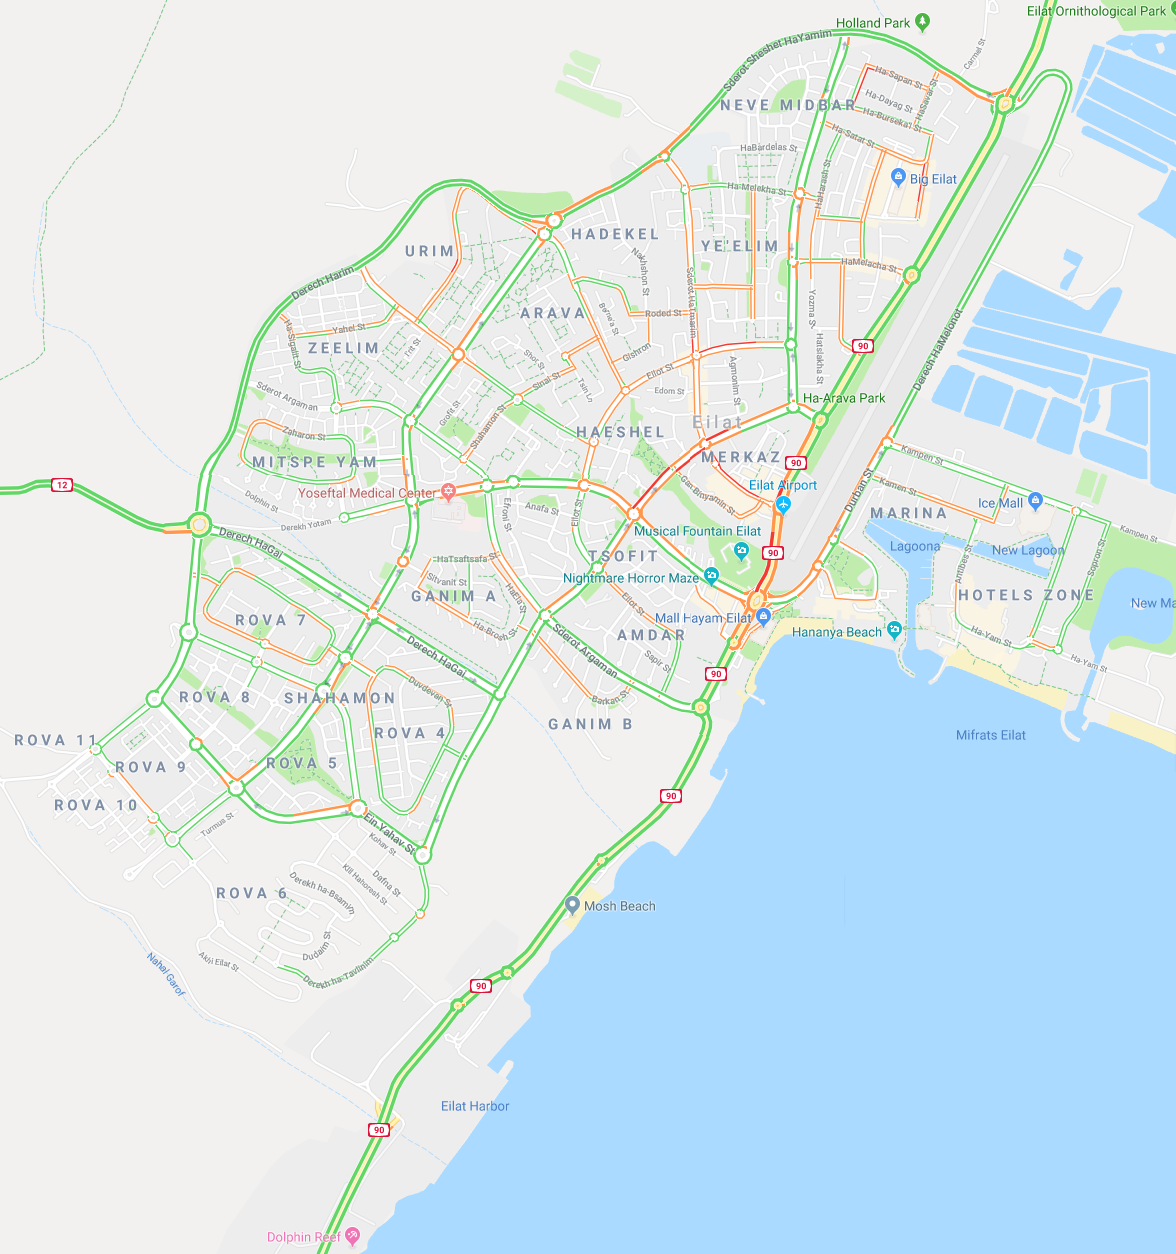
\includegraphics[scale=1]{eilat_traffic.png}
    \caption{Traffic map of Eilat at 5 PM weekdays (off-season)}
    \label{img:eilatTraffic}
\end{figure}

Israel's route 90 is the main road leading into Eilat, seen in the top right of figure \ref{img:eilatTraffic}, and is subject to heavy congestion during the tourism season, especially during peak hours. Red and orange roads indicate heavy and moderate congestion, respectively. During rush hours, congestion is moderate in most major city arteries even off-season. A notable hotspot is the Eilat airport (on the center right) which travelers frequently enter and exit. However, this airport is set to shut down as Ramon Airport opens later this year along route 90, and Ovda Airport (which feeds into route 12 on the far left) will stop handling civilian flights. This leaves Ramon airport as the only airport servicing Eilat, creating a focal point for congestion wherever route 90 meets with city roads. Given the already evident congestion, major traffic jams and increased travel times can be expected. 

\subsection{Tourism}[Joseph .]

Domestic tourism has larger impact on Israel’s tourism sector, accounting for 90\% of the bed nights spent in Eilat \cite{} With regard to the Ministry of Tourism’s spending, approximately 33\% of the budget is put toward marketing, 28\% is toward investment incentives, and 26\% for infrastructure investment. Israel’s most popular international markets include the United States, Russia, France, the UK, and Germany - accounting for nearly 50\% of the total number of tourists. In an attempt to draw more Europeans and Americans into Israel, the Open Skies Agreement in 2012 allowed direct flights to and from all EU countries. This agreement drove flight prices down and allowed more tourist flow to all parts of Israel. Within Eilat specifically, France and Russia as of 2015 represented the largest origin markets with a 42\% and 26\% claim respectively on international tourist arrivals, suggesting that this policy change increased potential tourism pull from the EU.



\subsection{Smart Cities}[Valeria K.?]

A smart city aims to ease the lives of its citizens by providing services as efficiently as possible. In order to do so they typically utilize innovative technologies that incorporate data analysis through the use of sensors and data collection. Cost, travel time, convenience, reliability, familiarity, weather, safety, environmental considerations, and existing infrastructure are factors that vary across cities and play a crucial role in understanding what citizens' needs and wants. Consequently, this information can then be used to determine which services should be prioritized. 

Existing smart city plans typically first incorporate a basic infrastructure of sensors, cameras, and city-wide WiFi in order to establish a constant flow of data. This data can be used in strategic ways to resolve the issues that are too dynamic and intricate to change via technology-neutral methods. These tools are installed through the city and reflect traffic flow, available parking, pedestrian traffic, etc. This information can be used to improve traffic flow by adjusting public transportation and traffic lights to real time demand. 

Successful smart cities across the world have several common factors, such as a strong commitment from government leaders that fosters the collaboration between the public sector and the private sector. Transparency, achieved by making collected data available to citizens, greatly increases confidence from citizens. Additionally, prioritizing continuous improvement is crucial due to rapidly changing technologies, since smart cities need to be constantly changing and adapting alongside them. 

Smart mobility, or Mobility as a Service (MaaS), aims to cause a fundamental shift in the traveler’s mentality by incentivizing customers with a cheaper, faster, and more convenient mode of transportation in comparison to traditional privately-owned vehicles. These services are created with the customer in mind and are ultimately used to target issues associated with the saturation of private vehicles including traffic congestion, road accidents, insufficient parking, and greenhouse gas emissions.

% Not sure if this should be a section of its own or how we should organize this
\section{Smart City Examples}
\subsection{Curitiba, Brazil}[Author?]
Curitiba is the capital of the state of Paraná in the south of Brazil. It has a population of about 1.8 million, making it Brazil’s 8th most populous city, and gets about two million tourists per year. During the 1970s there were a series of projects that focused on improving the city after it experienced incredibly rapid growth that led to overly congested streets. These were led by architect and three time mayor Jaime Lerner. The first project happened in 1972 and consisted of converting the main street in the center of the city to a pedestrian mall. The public objected to this, especially the shopkeepers, and in order to bypass this Lerner started construction a Friday evening after the courts had closed and made sure it was done within seventy-two hours. Public opinion rapidly shifted when they saw the benefits, instead requesting that the pedestrian zone be expanded. This was the beginning of an attitude change for all Curitiba, in terms of legislation and public opinion, that focused on bringing people together. Lerner adopted a philosophy of "act now, adjust later" as a means of avoiding Brazil’s bureaucracy in order to implement bold initiatives that would have likely been shut down or taken longer to carry out. Currently, 85\% of the population uses the bus system, given that it is the fastest and cheapest mode of transportation in the city. The incredibly efficient bus system known as Bus Rapid Transit (BRT) uses raised platforms and an electronic prepayment that allow for quicker stops, longer buses for a higher passenger capacity, and has five express bus avenues. The city has also made an effort to have large green areas and has a widely adopted recycling program. Due to its bold initiatives and successful implementation Curitiba is now recognized worldwide as a model for urban planning. 

\subsection{Freiburg, Germany}[Author?]
Freiburg, a city of about 220,000, suffered significant damage during World War II bombings, which led to a redevelopment of the inner areas during the reconstruction period. The population at the time prioritized their energy consumption and city layout over their private vehicles, suggesting that a viable solution would focus on city access rather than mobility. Planners also decided to place emphasis on supporting a diversity of cheap and clean transportation modes and services to adapt to user needs. With other considerations such as air pollution caused by traffic influencing the reconstruction of the city centre, ideas to address these issues involved pedestrianizing the city centre further to reduce the amount of cars being allowed inside. This city centre would be a hotspot for tourists containing restaurants, shops, and plenty of green space. Parking was made available directly outside the centre at a fee, and parking within the centre would get progressively more expensive - alleviating congestion in a tiered fashion. Before doing this the city ensured there was an efficient tram system, which when combined seamlessly with the bus system, was able to bring travelers within 7 minutes of the outskirts of the city. Since users were generally accepting of physical activity like walking and biking, the city also made an effort to expand its biking network by placing bikes next to tram/bus stations with parking available for cars as well. From 1984 to 2006, people using public transit increased by 100\% and a modal shift occurred when 9\% of the total population ditched private cars for their everyday travel needs.  By 2020, Freiburg is projected to have 29\% of travelers using private vehicles, 20\% using public transit, 27\% cyclists, and 24\% pedestrians. By reducing the stress on any one form of transportation, it should contribute to a well-balanced city-wide network for all users. Figure \ref{img:freiburg_modal_split} reflects the current and projected usage of the transportation network in Freiburg.

\begin{figure}[h]
    \centering
    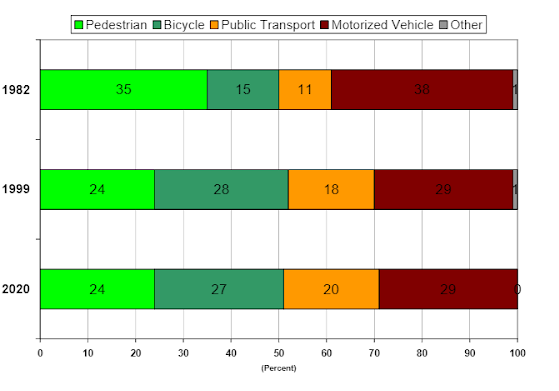
\includegraphics[scale=0.75]{freiburg_modal_split.png}
    \caption{Chart of Freiburg's transportation modal split over time.}
    \label{img:freiburg_modal_split}
\end{figure}

\subsection{Barcelona, Spain}[Author?]
Barcelona is the second largest city in Spain with 1.7 million residents, and it is considered to be one of the most densely populated european cities. It a popular tourist destination in Europe, and it sees about 8.2 million international visitors per year. Barcelona is widely recognized for its smart city initiatives, and has successfully implemented various smart city technologies. For example, there are sensors around the city that measure air quality as well as others that allow for street lights to be dimmed when there are no pedestrians in the area. Sensors were installed in public parks in order to decrease unnecessary water usage. Parking availability data is also collected through sensors and its displayed in a smart parking app that also allows for online payment. The city boasts a smart bus system with increased routes and with smart bus stops that include free wifi, charging stations and real life time updates of the bus schedule. It has an extensive bike-sharing program with about 180 km of bicycle lane. The city has a metro system that is 1.5 km per hour faster than the average car trip within the city. It will be implementing a ban on older vehicles, cars made before 1997 and trucks and vans made before 1994, in order to decrease air pollution in the city. Additionally, Barcelona is now implementing a plan to establish "Superblocks" through out the city. These are areas that encompass about nine blocks and prioritize pedestrians. Cars can circulate within the superblocks, but they have to do so at slow speeds, which will ideally lead to cars staying mostly within main roads. Overall, the super blocks aim to foster communities and increase life quality. Figure \ref{img:barcelona_superblock} shows a comparison of the current city layout and the proposed layout structure of superblock.

\begin{figure}[h]
    \centering
    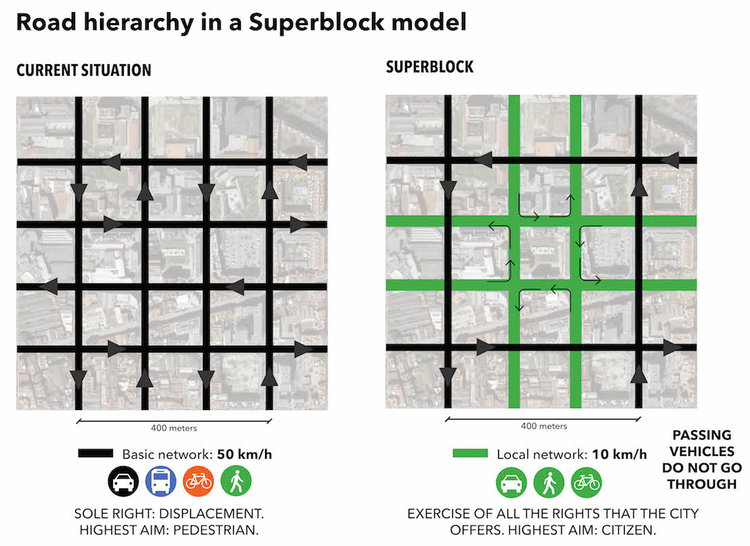
\includegraphics[scale=4.5]{barcelona_superblock.jpg}
    \caption{Diagram of Barcelona's "superblocks"}
    \label{img:barcelona_superblock}
\end{figure}

\subsection{Kansas City, United States}[Author?]
The Smart City Challenge asked mid-sized cities across the United States to provide a plan for moving to a brand-new transportation system that “would use data, applications, and technology to help people and goods move more quickly, cheaply, and efficiently" (*). Kansas City, Missouri had realistic objectives to create a higher quality of life, reduce traffic, and interconnect the city through smart technologies. Kansas City’s existing infrastructure was one of it’s most valuable assets, having the most highway miles in the region and the most established infrastructure of Fiber Optics and WiFi in the country at the time of the challenge. These resources eliminated the need for significant overhead and resources to build a network from scratch, which many other cities required. The city at the time was also emphasizing the use of bikes by implementing road diets and including a wayfinding app for bikers called RideKC. Though this was a start, Kansas City had 3 different plans laid out in their Smart City + Connected City proposal. Their plan entailed making improvements to underdeveloped areas in the East Side, introducing autonomous and connected vehicle technologies, as well as increasing connectivity sharing throughout the city. To address the East Side, they added a 3.5 km tram line which allowed easier transport the Center and East Side. They also added new wayfinding apps for pedestrians, and planned to increase their offerings for ride-sharing, bike-sharing, and city-wide wifi. In addition they began pilot tests for autonomous vehicles in a main artery within the city to test the viability of it expanding. These vehicles will also be connected to events, traffic, and could be implemented slowly while the infrastructure and policy-making develops. The city also plans to partner with ridesharing companies to obtain important real-time data, further expand the WiFi network to gather user data, and install information kiosks for travelers.

\subsection{Singapore}
The city-state of Singapore is one with a large population density, at nearly 8000 people per square kilometer. This issue is only expected to compound over time, with an estimated population of 6.9 million by the year 2030. However, the city believes it can be proactive in providing a livable city by using its largely technology-based economy and infrastructure to its advantage. Firstly, the city intends to make itself more pedestrian and biker-friendly by providing more bike lanes and pedestrian mobility services. Using autonomous cars, the city hopes to employ Mobility as a Service (MaaS) and reduce the amount of private vehicles on the road. Though autonomous cars can be difficult to test in a place with such a significant population density, it would alleviate major congestion areas and most likely reduce accidents, commute times, and allow for vehicle-to-vehicle (V2V) communications. Data gathered from these autonomous vehicles, cameras, sensors, and people on the city-wide network should be analyzed and redistributed to vehicles and travelers to adjust to real-time issues within the city. This system would save people money, time, and would make it easier for users to pay. Since vehicles take up 12\% of the city’s area, we can assume that constantly moving autonomous cars would significantly increase the amount of available city land previously held by parked private vehicles. Though Singapore has lofty goals, they hope to achieve full autonomous fleets in the next 10-15 years.

\subsection{Columbus, United States}
In 2015 Columbus, Ohio won the Smart City Challenge created by the U.S. Department of Transportation (DOT), which resulted in a \$50 million grant given to fund the city’s plans to create a smart transportation system. Additionally, it raised over \$500 million to support its smart city journey mostly by the city’s private sector. The collaboration between the public and private sectors has been crucial in Columbus' success in implementing its plan to transition into a smart city. It has installed sensors throughout the city that work to allow integrated data exchange (IDE) in order to decrease congestion and  have transportation be as smooth as possible. For example, this lets emergency vehicles to interact with traffic lights to decrease travel time. Columbus aims to convert to EVs and wants to decarbonize the city’s electric grid. It is also testing autonomous vehicles. It created a playbook in order to share project, case studies and strategies with other cities looking to implements smart city technologies.

\subsection{Summary}[Author?]
\begin{table}[h]
    \centering
    \small
    \begin{tabular}{ m{1.7cm} | m{1.1cm} | m{1.3cm} | m{3.4cm} | m{3.4cm} | m{3.4cm} }
        \textbf{City} & \textbf{Pop.} & \textbf{Area} & \textbf{Problem} & \textbf{Goal} & \textbf{Plan} \\
        \hline{}
        Curitiba, Brazil &
        1.76M &
        432km$^2$ &
        \begin{flushleft}Rapid population growth led to high congestion \end{flushleft} &
        \begin{flushleft}Provide better quality of life and transportation for citizens\end{flushleft} &
        \begin{flushleft}Pedestrian city center, bus rapid transportation, biking lanes, and green areas\end{flushleft} \\ 
        \hline{}
        
        Freiburg, Germany &
        227K &
        153km$^2$ &
        \begin{flushleft}Reconstruction after WWII \end{flushleft} &
        \begin{flushleft}Move away from car predominance, prioritize pedestrians\end{flushleft} &
        \begin{flushleft}Pedestrian city center, extend \& improve bike network, expand tram \& bus lines\end{flushleft} \\
        \hline{}
        
        Barcelona, Spain &
        1.6M &
        102km$^2$ &
        \begin{flushleft}High noise \& air pollution, saturated streets\end{flushleft} &
        \begin{flushleft}Move away from car predomincance, prioritize pedestrians\end{flushleft} &
        \begin{flushleft}Mini-superblocks, repurpose existing infrastructure, bike lanes, orthogonal bus network\end{flushleft} \\
        \hline{}
        
        Kansas City, US &
        489K &
        826km$^2$ &
        \begin{flushleft}Problem?\end{flushleft} &
        \begin{flushleft}Goal?\end{flushleft} &
        \begin{flushleft}Plan?\end{flushleft} \\
        \hline{}
        
        Singapore &
        5.6M &
        722km$^2$ &
        \begin{flushleft}High density \end{flushleft} &
        \begin{flushleft}Reduce private vehicles \end{flushleft} &
        \begin{flushleft}Autonomous taxis, data collection, improve ease of use\end{flushleft} \\
        \hline{}
        
        Columbus, Ohio &
        879K &
        578km$^2$ &
        \begin{flushleft}Problem?\end{flushleft} &
        \begin{flushleft}Goal?\end{flushleft} &
        \begin{flushleft}Plan?\end{flushleft}
    \end{tabular}
    \caption{Table of smart cities}
    \label{tab:smart_cities}
\end{table}

% Same as before with section headers, not sure how we should organize those
\section{Application of Global Smart Cities to Eilat: Advantages and Disadvantages}
These examples of cities show general trends in what solutions are being used to address similar problems. These examples range from smart city proposals and successful implementations to cities that tackled problems, such as congestion, through other solutions. Comparing these to Eilat’s characteristics is useful in understanding what could be implemented in Eilat, what constraints would be present, and how these can be adapted to Eilat. Through this scope the following advantages and disadvantages can be taken into consideration in regard to applying similar approaches to Eilat. 

Curitiba and Freiburg both implemented a pedestrian city center, which eliminated congestion within the city center. Eilat’s city center, unlike those of these two cities, is no concentric, which means that determining what zone to pedestrianised is more complicated. The location of the Ben Gurion Airport also poses an obstacle to developing a pedestrian center; however, given that this area will be repurposed in the coming years this is only a temporary constraint. An alternative to this is to extend the existing boardwalk along the water. This also helps address the extreme heat during the summer months. The sea provides a chilling factor that will encourage people wanting to walk outside, whereas an otherwise pedestrian city center might not be as effective as it has been in other cities with milder climates. Most of the cities that were studied made a conscious effort to promote cyclists by having bike sharing programs. Road diets do this by reducing the size of the roadways prioritize room for bike paths and pedestrian walkways. The mayor of Eilat (look for source) aims to promote a healthier and more athletic lifestyle for Eilat’s residents. Adjusting infrastructure in the city and offering services to promote walking and cycling is in the city’s best interest to accomplish this and decrease congestion. Once again, Israel’s climate must be taken into account and providing more shade throughout the city would further help address this issue. 

Investing in the improvement of public transportation has been incredibly beneficial to multiple cities such as Curitiba, Freiburg and Barcelona. Having bus/train/metro stops placed throughout the city so that citizens do not have a long transition from wherever they are located to the nearest bus stop has been key. Making sure waiting times are short is also important. Both of these factors motivate people to use public transportation instead of finding a different mode a transportation, and keeping the travel distances and waiting times short is especially important in Eilat due to the summer heat. 

Barcelona’s superblocks plan is aimed at a much larger city with a higher population density and higher pollution levels. This means that in order to implement it to a smaller city such as Eilat it would need to adapt to a much smaller scale. Perhaps a more practical approach would be to take specific characteristics of the superblock model and incorporate these into Eilat. Barcelona chose to gradually repurpose existing infrastructure to establish the superblocks instead majorly restructuring, which provides a smoother transition for residents.

%%% Not touched because it's unfinished
    ***pros and cons for singapore
-Pilot autonomous taxi fleets
-Collect and analyze real-time data using existing/future infrastructure
-Provide ease-of-use which will be unrivaled by personal vehicles

Cities that have struggled with congestion

London, England

San Francisco, California, USA

%%% End unfinished stuff?



\section{Smart City Tools}
\subsection{Sensors}[Author?]
A key component of smart cities are interconnected technologies that rely on sensors that collect data. This data is analyzed in real time and allows for immediate changes that result in improvements. The following lists the most common and useful sensor-based technologies found in smart cities world wide. 

\paragraph{Parking sensors} These are used to indicate available parking through and app that can also be used to pay for parking digitally.

\paragraph{Traffic light sensors} These track current traffic and adapt to data feed back in order to smooth traffic flow and decrease congestion. This is also known as smart traffic management.    
Emergency vehicles: A system can allow emergency vehicles to interact with traffic lights to provide quicker patient travel times.

\paragraph{Connected cameras} Installing cameras throughout a city and analyzing visuals can serve multiple purposes such as monitoring traffic, pinpointing crime, monitoring cleanliness of public spaces, registering crowd density and the movement of locally registered vehicles.

\paragraph{Street light sensors} These signal when there are no pedestrians in the area. When this is the case, street lights are dimmed for energy conservation.

\paragraph{Open data platform} Sharing collected data for transparency purposes fosters trust in government initiatives from citizens and can also be used by the private sector for innovative developments for the city, both of which contribute to the success of a smart city initiative.

\paragraph{Smart public transit} Adjust to real time demand and improves user friendliness by providing schedules that update to reflect real time arrivals and departures. 

\paragraph{Water sensors} Diminishes unnecessary water usage in public parks.

\paragraph{City-wide Wifi} Enables two-way data exchange between the city and travelers to aid in real-time adjustments

\paragraph{DRSC enabled vehicles} Dedicated short-range communication vehicles for either single or bidirectional connections with infrastructure and other vehicles from ranges of around 1 km. It was created for vehicles to increase driver safety and those surrounding the vehicle.

\subsection{Services}[Author?]
\paragraph{Shuttles/Bridj} Convenient method of strategically transporting people from point A to point B in mass without the hassle of a bus, train or subway system. It is used as a ridesharing service in some cities and can provide convenience to disabled and elderly users.

\paragraph{Ride-sharing} Transportation network companies (TNCs), such as Uber and Lyft, aim to provide on-demand transportation at a cost that is congruent to the ratio between consumer demand and the supply of drivers. The cost should also be agreed upon in advance.

\paragraph{Bike-sharing} Multiple startups provide stations with easy payment options to rent human-powered bikes and to combat the “last mile" issue. Cities have responded to interest in these by increasing bike infrastructure for riders.

\paragraph{Smart Hubs} Interactive and informational kiosks throughout the city that provide services such as free wifi, a charging station, city information, current weather, real time public transportation schedules, etc. 

\paragraph{Car-sharing} Companies like CAR2GO provide vehicles as others do bikes, allowing rentals without human intervention and rates including insurance, distance traveled, and time.

\paragraph{Streetcar/Subway system} Public examples in cities include a intra-city rail that operates often on a subscription or reloadable payment basis. They can be made less intrusive on existing if placed underground or if created to function in existing car lanes.

\paragraph{Bus system} The most ubiquitous public mode of transportation in cities without an underground rail system
Wayfinding apps for pedestrians/bikers: Provided by public and private companies to encourage the use of sustainable transportation options

\paragraph{SkyTran} An above-ground rail system which transports users in pods that fit two at speeds of up to 300 km/hr to their destination. Though it hasn’t been implemented, it is being developed in Tel-Aviv currently.

\paragraph{Autonomous Vehicles/Connected Vehicle Fleets} These have been piloted at level 4 autonomy (not full autonomy) in multiple cities to create interconnected taxi fleets which can simultaneously collect data for the city and communicate vehicle-to-vehicle (V2V).

\paragraph{Taxis/Gett} This service can be public or private, but it offers transportation at an agreed upon rate, which can vary based on traffic, time of day, or availability. It has an easy to use app interface or can be purchased in person. 

\paragraph{E-Scooters/E-Bikes} "Last mile" solutions for the rider who does not wish to pedal or push. They have rates based on distance traveled and time used, and often do not require specific pickup or dropoff infrastructure.

\paragraph{Trucking/Delivery Services} Any vehicle responsible for the transport of goods for commercial purposes

\paragraph{Vanpool/Carpool/Waze Carpool} Whether informal or through the use of available apps, the practice of commuting with others destined for the same, or a similar, location.

\paragraph{Paying online for public transportation}: Certain transportation networks have produced easy to use app/web interfaces in which travelers can purchase tickets across various modes of transportation.

\subsection{Policies}[Author?]
An important aspect of decreasing congestion and improving citizen quality of life is implementing policy changes. There are various city policies that have been designed specifically for this purpose, which can be taken as a basis. 

\paragraph{Congestion pricing} There is an imposed fee for entering a zone, typically the city center or the most congested area in the city. Some cities implement a fixed fee, while others have a fee that reflect the current congestion, when/where a vehicle is entering the zone and how long it is staying in it.

\paragraph{Restricted traffic zones} The city is divided into zones that are closed to traffic in varying levels. This can be determined in several ways, such as by time periods throughout the day/week, an entry-level based subscription, tiered fees based on proximity to center (number of cars inside), and plate number restrictions. Car entry can also be limited to residents, taxis, and emergency vehicles within designated zones, such as the city center. 

\paragraph{Parking restrictions} There are multiple ways to implement parking restrictions such as imposing a parking ban within the city center and having available parking outside of it. Having parking become incrementally pricier closer to the city center is another method. This can also be tied to the parking sensors that indicate real-time parking suggestion through an app.

\paragraph{Speed reductions} Severe reduction of speed limits within specific areas serve to accommodate bikers and pedestrians, as well as to discourage car usage within that area.

\paragraph{Subsidies} These are an effective economic incentive to promote specific behavior from consumers and citizens, such as using carpool options.

\paragraph{Road diets} The reduction of available vehicle driving space on roads to make bike lanes and pedestrian walkways available.

\paragraph{Waze Connected Citizens Program (CCP)} "The Waze Way of free data exchange, yielding actionable insights and improved mobility on a local and global scale."

\paragraph{Superblocks} Areas of about nine blocks that prioritize pedestrians with limited vehicle circulation. They aim to foster communities and increase life quality.

\subsection{Additional Technologies}[Author?]
\paragraph{Charging stations for electric vehicles (EVs)} Installing EV charging stations throughout the city to promote EV usage.

\paragraph{V2X communications} Combines V2V and vehicle-to-infrastructure (V2I) technology to become vehicle-to-everything, in which the vehicle communicates with all enabled devices within range.

% Organization?
\section{Goals for Eilat}
Based on the data gathered and analyzed regarding Eilat’s current situation, the determined problems and influencing factors, as well as the models and goals proposed by example cities the following goals would be good guidelines for Eilat for 2040:

\begin{enumerate}
    \item Transportation availability
    \begin{enumerate}
        \item Be within 300-500 meters of a bus stop
        \item Limit wait time to 10-15 minutes
    \end{enumerate}
    \item Decrease private vehicle usage
    \begin{enumerate}
        \item Residents: one vehicle per household
        \item Tourists: use other methods of transportation
    \end{enumerate}
    \item Establish mobility as a service
    \item Improve quality of life
    \begin{enumerate}
        \item Prioritize pedestrians and cyclists
    \end{enumerate}
\end{enumerate}


% Bibliography -- automatically managed in APA style, on a new page
\newpage
\bibliographystyle{apacite}
\bibliography{refs}

\end{document}
